\documentclass[aspectratio=169, handout]{beamer}

% PACKAGES -----------------------------------------------------------------------------------------

\usepackage{array}
\usepackage[export]{adjustbox}
\usepackage{caption}
\usepackage{listings}
\usepackage{ragged2e}
\usepackage{pgfplots}

\usetikzlibrary{patterns}

% THEMING ------------------------------------------------------------------------------------------

% Beamer slide structure
\usetheme{Madrid}
\setbeamertemplate{navigation symbols}{}
\setbeamertemplate{caption}[numbered]
\setbeamertemplate{caption label separator}[period]

% Beamer colors
\usecolortheme{beaver}
\setbeamercolor{item}{fg=darkred}
\setbeamercolor{section in head/foot}{bg = white}

% Beamer header
\addtobeamertemplate{frametitle}{\vspace{-0.2ex}}{\vspace{0.5ex}}
\setbeamercolor{frametitle}{fg=darkred,bg=}

% Beamer footer
\setbeamercolor{footer}{bg = white, fg = black}
\setbeamertemplate{footline}{
    \hbox{%
        \begin{beamercolorbox}[wd=.333333\paperwidth,ht=2.25ex,dp=1ex,left]{footer}
            \hspace{2ex}\insertshortauthor
        \end{beamercolorbox}%
        \begin{beamercolorbox}[wd=.333333\paperwidth,ht=2.25ex,dp=1ex,center]{footer}
            \insertshorttitle
        \end{beamercolorbox}%
        \begin{beamercolorbox}[wd=.333333\paperwidth,ht=2.25ex,dp=1ex,right]{footer}
            \insertframenumber\hspace{2ex}
        \end{beamercolorbox}
    }
}

% Code theming
\lstdefinestyle{codestyle}{
    language       = sql,
    keywordstyle   = \color{darkred},
    basicstyle     = \ttfamily\footnotesize,
    deletekeywords = {CLUSTER},
}

\lstset{style = codestyle}

% Other
\def\arraystretch{1.5}
\DeclareCaptionFont{darkred}{\color{darkred}}
\captionsetup{font=scriptsize,labelfont={darkred,scriptsize}}

% DOCUMENT INFORMATION -----------------------------------------------------------------------------

\title
    [High Performance Data Analysis 25/26]
    {\large Optimizing Deucalion's Automatic Report Generation}
\subtitle{\color{black} \small High Performance Data Analysis 25/26}

\author[Group 12]{
    \begin{tabular}{lc}
        Humberto Gomes & \color{gray} pg59806 \\
        José Lopes     & \color{gray} pg59807 \\
        José Soares    & \color{gray} pg60277
    \end{tabular}
}

\institute{
    Department of Informatics -- School of Engineering -- University of Minho \\
    \vspace{0.5\baselineskip}
    
\includegraphics[height=1cm]{res/SchoolOfEngineeringCropped.pdf}
}
\date{\scriptsize May 18\textsuperscript{th} 2026}

\newif\ifplacelogo
\logo{
    \ifplacelogo
        \begin{tikzpicture}[overlay, remember picture]
        \node[anchor=north east, inner sep = 0] at (current page.north east) {
            \LARGE
            
\includegraphics[height=1.1\baselineskip]{res/SchoolOfEngineeringCropped.pdf}
        };
        \end{tikzpicture}
    \fi
}

% DOCUMENT CONTENTS --------------------------------------------------------------------------------

\begin{document}

\placelogofalse
\frame[plain]{\titlepage}
\placelogotrue

\setcounter{framenumber}{0}
\justifying

\section{Introduction}

\begin{frame}{Introduction}
    \begin{minipage}{0.5\textwidth}
        \begin{itemize}
            \item The Deucalion Team generates periodical reports:
            \begin{itemize}
                \item Completed and failed jobs
                \item Compute hours per partition
                \item Jobs per partition
                \item ...
            \end{itemize}

            \vspace{0.5\baselineskip}
            \item Current Apache Spark implementation is slow and must be optimized
        \end{itemize}
    \end{minipage}
    \begin{minipage}{0.5\textwidth}
        \centering
        
\includegraphics[width = 0.7\textwidth]{/home/voidbert/ADED/TP1/report/res/DI.png}
    \end{minipage}
\end{frame}

\section{Methodology}

\begin{frame}{Methodology}
    \begin{itemize}
        \item Standard iterative profiling-oriented optimization methodology
    \end{itemize}

    \vspace{\baselineskip}
    \begin{minipage}{0.48\textwidth}
        \centering
        \textbf{System Metrics}
    \end{minipage}
    \hfill
    \begin{minipage}{0.48\textwidth}
        \centering
        \textbf{Apache Spark Metrics}
    \end{minipage}

    \begin{minipage}{0.48\textwidth}
        \centering
        \begin{tabular}{cl}
            
\includegraphics[width = 3ex, valign = c]{res/icons/Time.pdf}    &
            Runtime                                                          \\
            
\includegraphics[width = 3ex, valign = c]{res/icons/CPU.pdf}     &
            CPU usage                                                        \\
            
\includegraphics[width = 3ex, valign = c]{res/icons/HDD.pdf}     &
            Read and written bytes                                           \\
            
\includegraphics[width = 3ex, valign = c]{res/icons/Network.pdf} &
            Transmitted and received bytes
        \end{tabular}
    \end{minipage}
    \hfill
    \begin{minipage}{0.48\textwidth}
        \centering
        \begin{tabular}{cl}
            
\includegraphics[width = 3ex, valign = c]{res/icons/QueryPlan.pdf} &
            Query plans                                                        \\
            
\includegraphics[width = 3ex, valign = c]{res/icons/Tasks.pdf}     &
            Jobs, stages, and tasks                                            \\
            
\includegraphics[width = 3ex, valign = c]{res/icons/Shuffle.pdf}   &
            Shuffle reads and writes
        \end{tabular}
    \end{minipage}
    \vspace{\baselineskip}

    \begin{itemize}
        \item 48-thread runs on single nodes of Deucalion's ARM partition (Fujitsu A64FX)
        \item 5 warmup runs, 5 measurement runs
    \end{itemize}
\end{frame}

\section{Report Generator Implementations}

\begin{frame}{\texttt{Original} Report Generator}
    \begin{minipage}{0.5\textwidth}
        \centering
        Many query inefficiencies already optimized \\
        \vspace{0.5\baselineskip}
        \textbf{BUT} \\
        \vspace{0.5\baselineskip}
        Too many Spark actions (21)
    \end{minipage}
    \begin{minipage}{0.5\textwidth}
        \centering
        \includegraphics[width = 0.70\textwidth]{res/plans/original/4.pdf} \\
        \footnotesize Query plan for counting EuroHPC jobs per cluster
    \end{minipage}
\end{frame}

\begin{frame}[fragile]{\texttt{SinglePass} Report Generator}
    \begin{center}
        \textbf{Single Query}
        \vspace{\baselineskip}
    
        \begin{tabular}{c}
            \begin{lstlisting}
SELECT Period, cluster, Agency, COMPLETED, COUNT(*), SUM(totalJobSeconds)
    FROM jobs
    GROUP BY Period, cluster, Agency, COMPLETED\end{lstlisting}
        \end{tabular}

        \centering
        \vspace{\baselineskip}
        \textbf{Example Output Row}
        \vspace{\baselineskip}

    \begin{tabular}{
            |>{\tt\arraybackslash}l|
             >{\tt\arraybackslash}l|
             >{\tt\arraybackslash}l|
             >{\tt\arraybackslash}r|
             >{\tt\arraybackslash}r|
             >{\tt\arraybackslash}r|
        }

        \hline
        Period  & cluster & Agency & COMPLETED & COUNT(*) & sum(totalJobSeconds) \\ \hline
        Jan     & ARM     & EHPC   & COMPLETED &       10 &                 3600 \\ \hline
    \end{tabular}
    \end{center}
\end{frame}

\begin{frame}{Final Report Generators}
    \begin{minipage}{0.2\textwidth}
        \centering
        
\includegraphics[height = 0.45\textwidth]{res/frameworks/Spark.pdf}
    \end{minipage}
    \begin{minipage}{0.7\textwidth}
        \texttt{FastLoad}
        \begin{itemize}
            \item Fixed predefined schema
            \item Bulk CSV loading
        \end{itemize}
    \end{minipage}

    \vspace{1.5\baselineskip}

    \hspace{0.45\textwidth}
    \begin{minipage}{0.2\textwidth}
        \centering
        
\includegraphics[height = 0.5\textwidth]{res/frameworks/DuckDB.pdf}
    \end{minipage}
    \begin{minipage}{0.7\textwidth}
        \texttt{DuckDB}
        \begin{itemize}
            \item Direct port of \texttt{FastLoad}
        \end{itemize}
    \end{minipage}

    \vspace{1.5\baselineskip}

    \begin{minipage}{0.2\textwidth}
        \centering
        
\includegraphics[height = 0.5\textwidth]{res/frameworks/PostgreSQL.pdf}
    \end{minipage}
    \begin{minipage}{0.7\textwidth}
        \texttt{PostgreSQL}
        \begin{itemize}
            \item No bulk CSV loading support
            \item Direct port of \texttt{SinglePass}
        \end{itemize}
    \end{minipage}
\end{frame}

\section{Results}

\begin{frame}{Results -- Report Generator Performance}
    \vspace{0.5\baselineskip}
    \begin{minipage}{0.65\textwidth}
        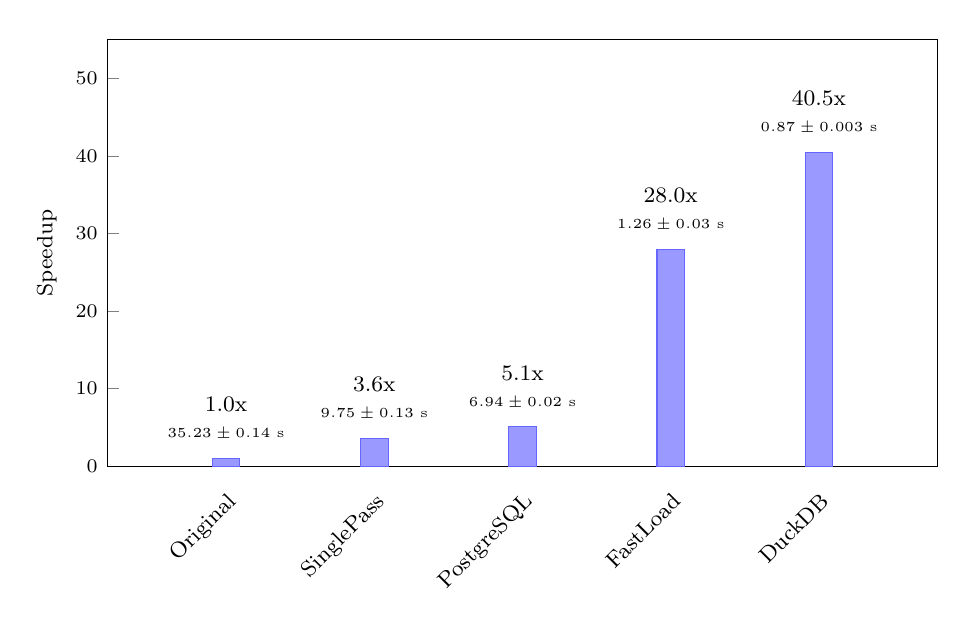
\begin{tikzpicture}
            \begin{axis}[
                ybar,
                width             = \textwidth,
                height            = 7cm,
                symbolic x coords = {
                    Original, SinglePass, PostgreSQL, FastLoad, DuckDB
                },
                xtick            = data,
                xtick style      = {draw = none},
                xticklabel style = {font = \footnotesize, rotate = 45, anchor = north east},
                enlarge x limits = 0.2,
                ylabel           = {Speedup},
                ymin             = 0,
                ymax             = 55,
                yticklabel style = {font = \scriptsize},
                ylabel near ticks,
                ytick pos = left,
                nodes near coords,
                point meta              = explicit symbolic,
                nodes near coords style = {font = \footnotesize, align = center, yshift=3pt},
                ylabel style            = {font = \footnotesize}
            ]
                \addplot[fill = blue!40, draw = blue!60] coordinates {
                    (Original,    1.00) [1.0x  \\ \tiny $35.23 \pm  0.14$ s]
                    (SinglePass,  3.61) [3.6x  \\ \tiny $ 9.75 \pm  0.13$ s]
                    (PostgreSQL,  5.07) [5.1x  \\ \tiny $ 6.94 \pm  0.02$ s]
                    (FastLoad,   27.96) [28.0x \\ \tiny $ 1.26 \pm  0.03$ s]
                    (DuckDB,     40.46) [40.5x \\ \tiny $ 0.87 \pm 0.003$ s]
                };
            \end{axis}
        \end{tikzpicture}
    \end{minipage}
    \hspace{-0.05\textwidth}
    \begin{minipage}{0.35\textwidth}
        \vspace{-3.25\baselineskip} % At this point, I only care about getting this centered
        \begin{itemize}
            \item \texttt{Original} $\rightarrow$ \texttt{SinglePass}: \\
                  \small 83\% reduction in disk reads
            \vspace{\baselineskip}
            \normalsize
            \item \texttt{SinglePass} $\rightarrow$ \texttt{FastLoad}: \\
            \begin{center}
                \small
                \vspace{\baselineskip}
                26 stages, 61 tasks \\
                $\downarrow$ \\
                2 stages, 25 tasks
                \vspace{\baselineskip}
            \end{center}
            \item \texttt{DuckDB} and \texttt{PostgreSQL}: \\
                  \small Different frameworks
        \end{itemize}
    \end{minipage}
\end{frame}

\begin{frame}{Results -- Methodological Problems}
    \begin{itemize}
        \item Unrealistic methodology (no Spark init time, JVM warmup, page cache, \ldots)
        \item Cannot capture best-case Spark performance
    \end{itemize}

    \begin{center}
        \begin{tikzpicture}
            \begin{axis}[
                % Graph properties
                ybar,
                x         = 4pt,
                bar width = 4pt,
                height    = 0.4\textwidth,
                % X axis
                xlabel           = {\texttt{FastLoad} Run},
                xticklabel style = {font = \scriptsize},
                xtick pos        = bottom,
                xlabel near ticks,
                % Y axis
                ylabel           = {Runtime (s)},
                yticklabel style = {font = \scriptsize},
                ymin             = 0,
                ymax             = 2,
                ytick pos        = left,
                ylabel near ticks,,
                % Font size (will not take effect if place earlier)
                xlabel style = {font = \footnotesize},
                ylabel style = {font = \footnotesize}
            ]

                \draw [pattern = north east lines] (axis cs:5, 0) rectangle (axis cs:10, 2);

                \addplot[fill = blue!40] table [x expr = \coordindex + 0.5, y = TIME]
                    {res/results/treated/Warmup.csv};

                \draw [red, thick] (axis cs:0, 1.2558) -- (axis cs:60, 1.2558);
                \node [red] at (axis cs:60, 1.35) {\small $\bar{t}$};
            \end{axis}
        \end{tikzpicture}
    \end{center}
\end{frame}

\section{Conclusions}

\begin{frame}{Conclusions}
    \centering
    Use the right tool for the job
    \vspace{1.5\baselineskip}

    \begin{minipage}[t]{0.25\textwidth}
        \centering
        
\includegraphics[height = 0.45\textwidth]{res/frameworks/Spark.pdf} \\
        \vspace{0.5\baselineskip} \texttt{SinglePass} \\
        \textbf{3.6$\times$ speedup} \\
        \vspace{0.5\baselineskip} \small \color{gray} No compromises
    \end{minipage}%
    \begin{minipage}[t]{0.25\textwidth}
        \centering
        
\includegraphics[height = 0.45\textwidth]{res/frameworks/Spark.pdf} \\
        \vspace{0.5\baselineskip} \texttt{FastLoad} \\
        \textbf{28.0$\times$ speedup} \\
        \vspace{0.5\baselineskip} \small \color{gray} No schema inference
    \end{minipage}%
    \begin{minipage}[t]{0.25\textwidth}
        \centering
        
\includegraphics[height = 0.5\textwidth]{res/frameworks/DuckDB.pdf} \\
        \vspace{0.5\baselineskip} \texttt{DuckDB} \\
        \textbf{40.5$\times$ speedup} \\
        \vspace{0.5\baselineskip} \small \color{gray} Platform change
    \end{minipage}%
    \begin{minipage}[t]{0.25\textwidth}
        \centering
        
\includegraphics[height = 0.5\textwidth]{res/frameworks/PostgreSQL.pdf} \\
        \vspace{0.5\baselineskip} \texttt{PostgreSQL} \\
        \textbf{5.1$\times$ speedup} \\
        \vspace{0.5\baselineskip} \small \color{gray} ACID guarantees
    \end{minipage}
\end{frame}

\placelogofalse
\frame[plain]{\titlepage}
\placelogotrue

\end{document}
